\chapter{Introduzione}
\label{cap:introduzione}

% Introduzione al contesto applicativo.\\

% \noindent Esempio di utilizzo di un termine nel glossario \\
% \gls{api}. \\

% \noindent Esempio di citazione in linea \\
% \cite{site:agile-manifesto}. \\

% \noindent Esempio di citazione nel pie' di pagina \\
% citazione\footcite{womak:lean-thinking} \\
\intro{Il seguente capitolo vuole introdurre brevemente l'azienda con il relativo contesto aziendale e l'organizzazione del testo con le norme tipografiche adottate.}\\


\section{L'azienda}

THRON S.p.A è un'azienda italiana con sede a Piazzola sul Brenta specializzata nello sviluppo di SaaS (Software as a Service).
I suoi prodotti principali sono la THRON DAM Platform e il THRON PIM. 
Il primo è una piattaforma nata con l'obiettivo di gestire, organizzare e distribuire i contenuti digitali di un'azienda.
Il THRON Pim invece è una soluzione per la gestione delle informazioni sui prodotti, che si concentra
sulla raccolta, organizzazione e distribuzione delle informazioni relative ai prodotti di un'azienda.\\
In sintesi, il primo prodotto si concentra sulla gestione dei contenuti digitali, il secondo invece
si focalizza sulla gestione delle informazioni sui prodotti.
L'obiettivo è garantire una gestione centralizzata dei contenuti e semplificarne l'adattamento e la distribuzione su diversi
canali in modo efficiente.
All'interno dell'azienda, l'area R\&D è suddivisa in due team: il team Prodotti, responsabile della gestione
del PIM, e il team Contenuti, focalizzato sulle tematiche legate al DAM.\\
Durante il mio stage presso l'azienda, sono stato inserito come sviluppatore frontend all'interno dell'area Prodotto, nel team Prodotti.

\section{Metodologie di sviluppo}
Nel contesto aziendale di THRON, vengono adottate metodologie di sviluppo agile per garantire un'efficace
gestione dei progetti. La filosofia Agile pone un forte focus sulla collaborazione tra i membri del team,
sulla capacità di rispondere in modo rapido ai cambiamenti, nonchè sull'orientamento al cliente e alla consegna di prodotti qualitativi.\\
Il framework Scrum, parte integrante dell'approccio Agile, è utilizzato all'interno dell'azienda per organizzare il lavoro in iterazioni chiamate
`Sprint' della durata di due settimane ciascuna. Questo approccio a breve termine consente al team di concentrarsi su attività specifiche, pianificando
e completando le attività in maniera incrementale.\\
% Al termine di ogni Sprint è prevista una revisione dei risultati ottenuti e un'opportunità 
% di riflessione per migliorare le prestazioni del team nelle settimane successive.\\
Al termine di ogni Sprint vengono organizzate molteplici riunioni: `Sprint Review', in cui il team presenta i risultati ottenuti durante lo Sprint,
`Sprint Planning', in cui vengono pianificate le attività da svolgere durante lo Sprint successivo e `Sprint Retrospective', in cui il team riflette sulle prestazioni del team e sulle possibili migliorie.\\
L'importanza della comunicazione e della condivisione delle informazioni è supportata dalla pratica quotidiana della riunione `Daily Scrum', durante la quale
ogni membro del team esprime il proprio progresso, eventuali ostacoli e le prossime attività pianificate. Questa pratica aiuta a mantenere l'allineamento e
la trasparenza, nonché a individuare tempestivamente eventuali problemi da risolvere.\\
Le riunioni settimanali chiamate `Competence' rappresentano un'altra componente importante adottata da THRON. Riunendo i membri dello sviluppo 
che condividono la stessa area di competenza, come front-end o back-end, queste riunioni offrono un'opportunità di scambio di conoscenze e di valutazione dei progressi.
\section{Strumenti di sviluppo}
Durante l'esperienza di stage presso THRON, l'utilizzo di una varietà di strumenti di sviluppo è stato fondamentale per assicurare un processo di lavoro efficiente.\\
Di seguito, sono elencati gli strumenti che sono stati impiegati per lo sviluppo del progetto:

\begin{itemize}
  \item \textbf{Teams}: per le comunicazione sia asincrone che sincrone con il team;
  \item \textbf{Microsoft 365} per la gestione della mail aziendale;
  \item \textbf{Jira} per il tracciamento e la gestione delle attività assegnate durante il periodo di stage (esempio in figura \ref{fig:board-jira});
  \item \textbf{AWS} per la gestione della repository del mio progetto, per la build e per il deploy dello stesso;
  \item \textbf{Fork} per la gestione del versionamento del codice sorgente;
  \item \textbf{Postman} per la creazione, esecuzione e test delle chiamate verso gli endpoint creati durante lo sviluppo;
  \item \textbf{Confluence} per la creazione e gestione della documentazione relativa al progetto di stage;
  \item \textbf{StarUML} per la modellazione dei casi d'uso.
\end{itemize}

\begin{figure}[!ht] 
  \centering 
  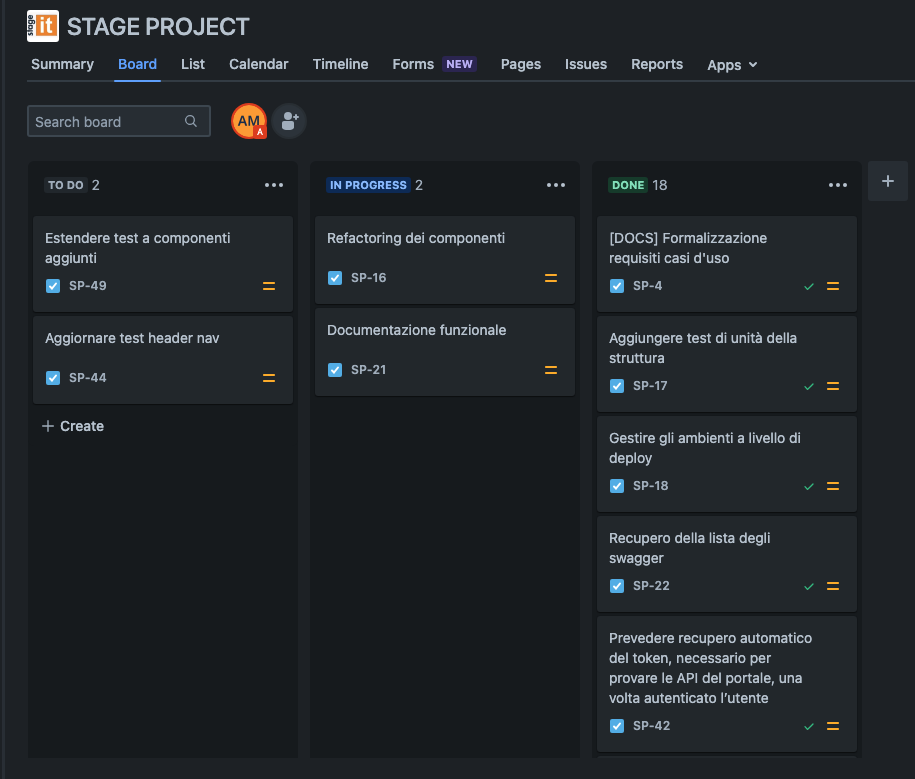
\includegraphics[width=0.9\columnwidth, alt={Esempio di utilizzo della board di Jira}]{images/Board.jpg}
  \caption{Board Jira}\label{fig:board-jira}
\end{figure}

\section{Organizzazione del testo}
\begin{description}
    \item[{\hyperref[cap:descrizione-stage]{Il secondo capitolo}}] descrive il progetto svolto durante il periodo di stage, mettendo in risalto gli obiettivi imposti dall'azienda e i possibili rischi.
    \item[{\hyperref[cap:analisi-requisiti]{Il terzo capitolo}}] descrive l'analisi dei requisiti del progetto di stage attraverso la modellazione dei casi d'uso e l'estrapolazione dei requisiti partendo da essi.
    \item[{\hyperref[cap:progettazione-codifica]{Il quarto capitolo}}] approfondisce le tecnologie utilizzate per lo sviluppo del progetto e descrive le scelte progettuali effettuate, descrivendo poi le attività di codifica.
    \item[{\hyperref[cap:verifica-validazione]{Il quinto capitolo}}] descrive le attività di verifica e validazione, descrivendo i test effettuati e i risultati ottenuti.
    \item[{\hyperref[cap:conclusioni]{Il sesto capitolo}}] presenta le conclusioni tratte dallo stage, esponendo le conoscenze acquisite, le competenze sviluppate e le considerazioni personali. 
\end{description}

\clearpage

Riguardo la stesura del testo, relativamente al documento sono state adottate le seguenti convenzioni tipografiche:
\begin{itemize}
  \item Gli acronimi, le abbreviazioni e i termini ambigui o di uso non comune, menzionati nel documento, vengono definiti all'interno del glossario alla fine del seguente documento;
  \item I termini in lingua straniera o facenti parte del gergo tecnico sono evidenziati con il carattere corsivo;
  \item Ogni termine presente nel glossario, è contrassegnato dalla lettera `G' come apice.
\end{itemize}
% Riguardo la stesura del testo, relativamente al documento sono state adottate le seguenti convenzioni tipografiche:
% \begin{itemize}
% 	\item gli acronimi, le abbreviazioni e i termini ambigui o di uso non comune menzionati vengono definiti nel glossario, situato alla fine del presente documento;
% 	\item per la prima occorrenza dei termini riportati nel glossario viene utilizzata la seguente nomenclatura: \emph{parola}\glsfirstoccur;
% 	\item i termini in lingua straniera o facenti parti del gergo tecnico sono evidenziati con il carattere \emph{corsivo}.
% \end{itemize}
